\documentclass[11pt,a4paper]{article}

\usepackage[utf8]{inputenc}
\usepackage{graphicx}
\usepackage{wrapfig}
\usepackage{color}
\usepackage{amsmath}
\usepackage{amssymb}
\usepackage[inkscapelatex=false]{svg}
\usepackage{array, makecell}
\usepackage{mhchem}
\usepackage{tabularx}
\usepackage{braket}
\usepackage{pdfpages}
\usepackage{svg}

\usepackage{multicol}
\usepackage{colortbl}
\usepackage[Export]{adjustbox}
\adjustboxset{max size={0.9\linewidth}{0.9\paperheight}}
\usepackage[colorlinks=true,linkcolor=red,citecolor=green]{hyperref}

\textwidth=16cm
\textheight=23cm
\topmargin=-2cm
\oddsidemargin=0cm

\setlength{\parindent}{0em}
\setlength{\parskip}{0.6em}
\setlength{\jot}{12pt}

\renewcommand{\arraystretch}{1.4}
\renewcommand\theadfont{\bfseries}

\newcommand{\todo}[1]{\textcolor{red}{TODO: #1}}

\begin{document}

\title{Ising model on random graphs with non-limited range of interactions}
\author{Dawid Karpiński,\\Supervisor: dr inż. Krzysztof Suchecki}
\date{}
\maketitle

\section*{Abstract}

The Ising model, renowned for its simplicity and effectiveness in capturing phase transitions, serves as a powerful tool to analyze the emergent properties of complex systems. The core objective of this research is to unravel the implications of non-limited interaction ranges in the context of random graphs. Traditional Ising models often assume a fixed range of interactions among neighboring spins. This work challenges that assumption by considering scenarios where interactions extend beyond the nearest neighbors, incorporating a broader and more realistic perspective on the interplay between spins.

\section{Introduction}

Historically, the Ising model has played a crucial role in the development of statistical mechanics and the understanding of critical phenomena. The starting point - one-dimensional Ising model - was solved exactly by Ernst Ising's advisor, Wilhelm Lenz, in 1920. However, the two-dimensional case remained unsolved for many years until the solution has been found independently by Lars Onsager in 1944, marking a significant breakthrough.


\subsection{The Ising model}

It serves as a basic model for understanding phase transitions in physical systems. In its simplest form, the model considers a lattice of discrete spins, that represent magnetic moments. These spins can be either "up" (+1) or "down" (-1), corresponding to the two possible magnetic states $s_{ij}\in\{-1, +1\}$.

The energy of the system is determined by the interactions between neighboring spins. The model assumes that each spin interacts with its nearest neighbors, and the total energy of the system depends on the alignment of these spins relative to each other.

The Hamiltonian $H$ of such model can therefore be described as:

\begin{equation}
    H = -\frac12\sum_{\langle i,j \rangle} J_{ij} s_i s_j + \mu\sum_i h_i s_i
\end{equation}

When analyzing the model without any magnetic field ($B=0$), only the first term remains.

Depending on the sign of an interaction constant $J$, the evolution of the system differs. Hence, in case of $J>0$ (ferromagnetic interaction), if neighboring spins are aligned in the same direction the energy is lowered, and if they are aligned oppositely the energy is increased. However, when $J<0$, indicating an antiferromagnetic interaction, the dynamics of the model undergo a reversal.

\subsection{The mean-field solution}

A useful tool that we used for the analytical calculations is the mean-field theory. 

\subsection{Random graphs}

The Ising model has been successively extended and applied to various disciplines beyond physics. There exist various ways of extending the model.

One could for instance change the topography of the spin lattice. By employing the Ising model on random graphs, one can study e.g. how information spreads through a social network, shedding light on the mechanisms that govern the diffusion of ideas, opinions, or trends within these complex systems. This approach not only contributes to the understanding of social dynamics but also showcases the versatility of the Ising model in capturing the essence of diverse real-world scenarios.

\begin{figure}[ht!]
    \centering
    \includegraphics[width=\linewidth]{../figures/ER_graph.pdf}
    \caption{Examples of generated ER networks}
\end{figure}


For this thesis, I have chosen to focus my analysis on an Erdős-Renyi graph $G_{N,p}$. Such network is constructed by choosing a number of edges for each node, with some probability described by a parameter $p$. Moreover, the average number of nearest neighbors for each node is given by the following equation:

\begin{equation}
    \braket{k} = (N-1) \cdot p
\end{equation}

\todo{mean-field}

\todo{general solution to mean field}


\section{Motivation}

In real-world scenarios, interactions typically diminish swiftly as distance increases. However, within complex networks, particularly in random or complex graphs, the number of neighbors grows rapidly with distance. This contrast serves as a motivation to explore the implications of such connectivity patterns within complex systems.

To systematically explore this phenomenon, we therefore adopt the assumption of exponential decay in interaction strength with distance. Simultaneously, we are aware of the rapid growth in the count of neighbors with increasing sizes of the complex networks.

Hence we recognize the potential significance of such long-range interactions between distant nodes, contrary to the typical neglect of such influences in models of physical systems.


\section{Literature review}

Several works were found that include similar fields of study. 
Simulation of Ising model on small-networks ...


\section{Analytical mean-field approximation for critical temperature}

For the purpose of a comparative analysis, we derived a formula that is based on the mean-field approximation was derived. To start with, we assume that interaction strength between spins undergoes exponential decay over longer distances, denoted by $l$. This decay can be represented as $\exp[-\alpha (l-1)]$. The parameter $\alpha$ was added for better control over the decay speed.

Since we consider a model with unlimited, long-range interactions, the sum of all neighbors at a given distance is equal to the total number of spins, $N$. We can approximate, that root spin will have $\braket{k}=k$ neighbors and at each consecutive path length, $(k-1)$. Therefore, we can write such sum as

\begin{equation}\label{eqn:N_l}
    N = \sum_{l=1}^{l_{\max}} N_l = \sum_{l=1}^{l_{\max}} k (k-1)^{(l-1)}.
\end{equation}

The formula \eqref{eqn:N_l} is a finite geometric series, which can be simplified into

\begin{equation}\label{eqn:geom_series}
    N = k \sum_{l=1}^{l_{\max}} (k-1)^{(l-1)} = k\frac{(1 - q^{l_{\max}})}{(1 - q)},\ \text{where}\ q=k-1.
\end{equation}

Then, by using the above, we can obtain a formula for maximum path length, $l_{\max}$, in the ER graph as

\begin{equation}\label{eqn:l_max}
    l_{\max} = \log_{(k-1)}{\left[N\frac{(k-2)}{k} + 1\right]}.
\end{equation}

Based on the general mean-field solution, the critical temperature, $T_C$, is given by

\begin{equation}\label{eqn:base_tc}
    k_B T_C = J \sum_{l=1}^{l_{\max}} N_l~ e^{-\alpha (l-1)} = kJ \sum_{l=1}^{l_{\max}} \left[e^{-\alpha}(k-1)\right]^{(l-1)},
\end{equation}

which once more is a geometric series. Similar to \eqref{eqn:geom_series}, the equation \eqref{eqn:base_tc} can be simplified, but this time with the common ratio of $q=e^{-\alpha}(k-1)$.

When we make $k_B=1$, $J=1$ and use \eqref{eqn:l_max}, the final analytical mean-field formula for the critical temperature, $T_C$, is

\begin{equation}
    T_C = \frac{1 - [e^{-\alpha}(k-1)]^{\log_{(k-1)}{\left[N\frac{(k-2)}{k} + 1\right]}}}{1 - e^{-\alpha}(k-1)}.
\end{equation}

The key point that emerges, following the above derivation, is that there are two distinct regions of behavior of the system. The sum in \eqref{eqn:base_tc} converges only when $|q|<1$, thus when $\exp[\alpha] > (k-1)$.

Therefore, we find the equation describing boundary separating those regions to be

\begin{equation}
    e^\alpha = k-1.
\end{equation}

\section{Simulation}

\subsection{Path generation models for the spin interactions}

When generating interaction matrix from edges of a given Erdős-Renyi graph, we explored different models for finding paths between spins, including the ones of long-range.

Initially, we considered a model where two spins can interact with each other through multiple connections. This could possibly be achieved by raising the adjacency matrix $A=[a_{ij}]$ of a graph to some set power. For a given power $l$, $A^l$ will result in a new matrix in which each item represents the number of walks of length $l$ between the $i$-th and $j$-th spin.

However, this approach raised concerns regarding potential overestimation of interaction counts. The cumulative nature of matrix powers could lead to an inaccurate representation of the actual connectivity between spins. Self-loops in the graph could also contribute to the growth of matrix powers and their impact might be disproportionate. Additionally, selecting an inappropriate power may again yield misleading insights. These issues prompted a reevaluation of our strategy.

Therefore, we opted for a more precise approach, which was the usage of Breadth-First Search (BFS) algorithm to find the shortest path of a chosen length. This way, two given spins interact with each other exclusively through a single connection.

\begin{figure}[ht!]
    \centering
    \caption{\textbf{Path generation methods comparison}}
    \includegraphics[width=\linewidth]{../figures/single_vs_multiple.pdf}
\end{figure}
\pagebreak


\subsection{The simulation algorithm}

In order to perform the simulation, we used Metropolis algorithm. It consists of the following steps:
\begin{itemize}
\item Generate the ER graph with a probability parameter $p$ and $N$ spins, each initialized with a random value of either +1 or -1.
\item Repeat until the set number of steps has been reached:
    \begin{itemize}
    \item Take a randomly selected spin $s$ with a uniform probability $\mathbb{P}(s)=1/N$.
    \item Calculate the change in system's energy as $dE = 2 s \sum\limits_{\braket{i,j}}^\text{neighbors} J_{ij} s_j$
    \item If $dE\leq0$, we flip the spin, else if $dE>0$, we flip only when $x < \exp[-dE/T]$ is satisfied (where $x$ is a random number, drawn from range $[0,1]$)
    \end{itemize}
\end{itemize}

During one time step ($N$ iterations), each spin will be flipped, on average, at least once.

For the first 0-30 time steps, with temperatures lower than the critical $T_C$, the system tends towards equilibrium. For larger than $T_C$ however, it typically oscillates around some value.

We show this in the figure \ref{fig:mag_vs_time} by looking at how magnetization changes with time step. In this case, for the highest temperature $T=100$, it fluctuates around zero, indicating a state in which approximately half of the spins are pointing up and the other half are pointing down.

\begin{figure}[ht!]
    \centering
    \caption{\textbf{Magnetization vs. time step}}
    \includegraphics[width=\linewidth]{../figures/magnet_vs_steps.pdf}
    \label{fig:mag_vs_time}
\end{figure}

\subsection{Results and Discussion}

\begin{figure}[ht!]
    \centering
    \caption{\textbf{Energy and Magnetization vs. time step}}
    \includegraphics[width=\linewidth]{../figures/energy_magnet_vs_temp.pdf}
\end{figure}


\section{Conclusion}

\begin{figure}[ht!]
    \includegraphics[width=\linewidth]{../figures/suscept_ER_nearest.pdf}
\end{figure}


\begin{figure}[ht!]
    \includegraphics[width=\linewidth]{../figures/suscept_ER_single.pdf}
\end{figure}

\todo{$T_C$ vs. k with n kept constant}
\begin{figure}[ht!]
    \includegraphics[width=\linewidth]{../figures/TC_vs_alpha.pdf}
\end{figure}

\todo{$T_C$ vs. $\alpha$ for exponential decay}
\begin{figure}[ht!]
    \includegraphics[width=\linewidth]{../figures/TC_vs_size.pdf}
\end{figure}

\begin{figure}[ht!]
    \includegraphics[width=\linewidth]{../figures/TC_vs_k.pdf}
\end{figure}

\todo{$e^{-\alpha k}$ vs. $1/k^\alpha$}

\begin{figure}[ht!]
    \centering
    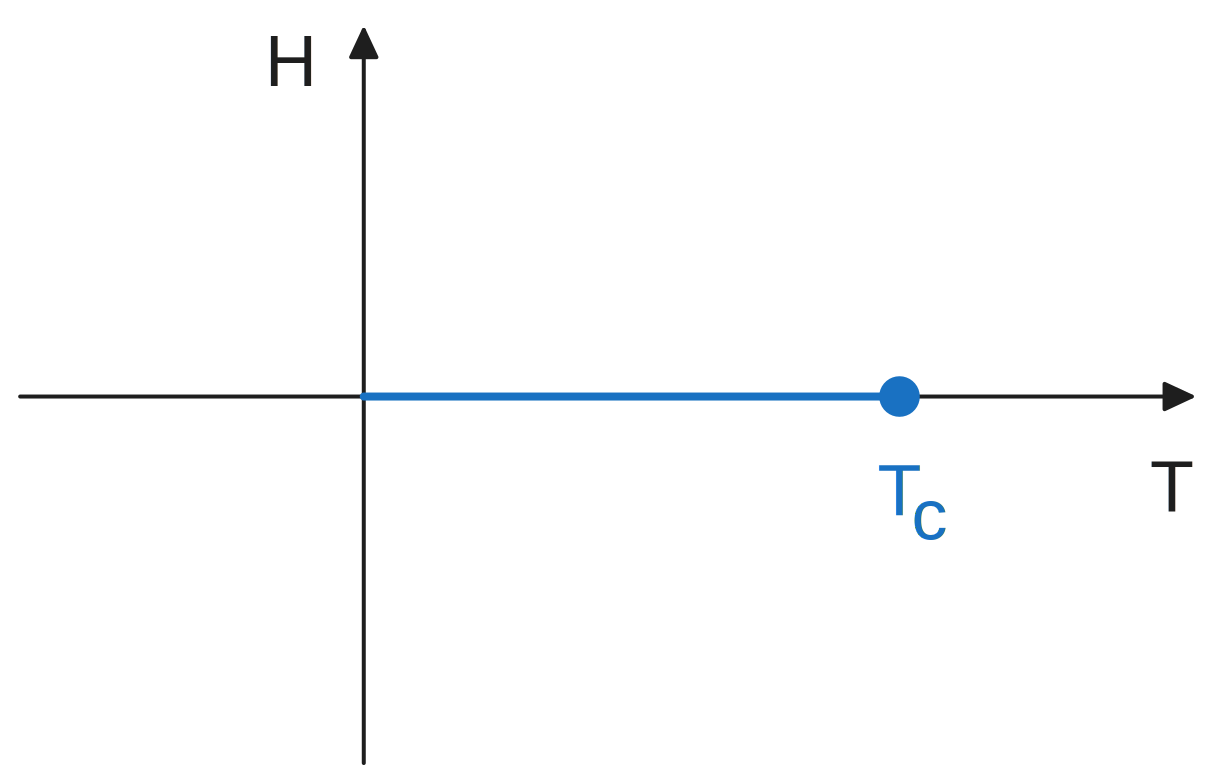
\includegraphics[width=0.7\linewidth]{../figures/phase-diagram.pdf}
\end{figure}

\end{document}
